\documentclass[twoside,11pt]{article}

\usepackage{jsat}
\input epsf
\special{papersize=8.5in,11in}

%\jsatheading{1}{2004}{25-30}
\ShortHeadings{Accelerated Deletion-based Extraction of Minimal Unsatisfiable Cores }
{Alexander Nadel, Vadim Ryvchin and Ofer Strichman}
%\firstpageno{25}


%\usepackage{amsfonts,epsfig}
\usepackage{algorithm}
\usepackage{algorithmicx}
\usepackage[noend]{algpseudocode}
\usepackage{xspace}
%\usepackage{epsfig}
\usepackage{color}
\usepackage{amsfonts}
\usepackage{graphicx}

\newcommand\muser{\tool{MUSer2}\xspace}
\renewcommand\square{\bot}
\newcommand\haifamuc{\tool{HaifaMUC}\xspace}
\newcommand\haifahlmuc{\tool{HaifaHLMUC}\xspace}
\newcommand\muserabr{\tool{Minisatabb}\xspace}
\newcommand\xvsmuser{2.18x\xspace}
\newcommand\tvsmuser{13\xspace}
\newcommand\xvsabr{48\%\xspace}
\newcommand\tvsabr{4\xspace}
\renewcommand\Pr{\pi}

\newcommand\qed{\hfill\hbox{\hskip 4pt
                \vrule width 3pt height 1pt depth 1pt
                \hbox{\vrule width 2pt height 3.5pt depth 1pt}}}

\newtheorem{example}{Example}

\begin{document}

% Macros
\newcommand\limply{\rightarrow}
\newcommand\type[1]{{\tt #1}}
\newcommand\nin{\noindent}
\newcommand\true{\mbox{{\sc true}}\xspace}
\newcommand\false{\mbox{{\sc false}}\xspace}
\newcommand\comment[1]{}
%\newcommand\note[2]{\begin{itemize} \item[$\Diamond$ \emph{Side-Note $\rangle$}] {\bf #1: }#2 $\Diamond$\end{itemize}}
\newcommand\brackets[1]{\vspace{0.5 cm}\begin{center}#1\end{center}\vspace{0.3 cm}}
\newcommand\alg[1]{{\sc #1}}
\newcommand\margin[1]{\marginpar{\fbox{#1}}}
\newcommand\first[2]{\margin{#2}\label{page:#1}}
\newcommand\graph[2]{\begin{figure} \begin{center}\scalebox{0.7}{\input{#1.pstex_t}}\caption{\label{fig-eq:#1}#2}\end{center}\end{figure}}
\newcommand\tool[1]{{\sc #1}}

% eq specific macros



\newcommand\E{\mbox{\tiny E}} % for superscript E
\newcommand\eq{\varphi^{\E}} % Equality formula (after reduction)
\newcommand\peq{{\psi^{\E}}}  % Equality formula (after reduction)
\newcommand\equf{\varphi^{\mbox{\tiny UF}}}% Equality formula with uninterpreted functions (before reduction)
\newcommand\eqfc{consistent^{\E}} % Functional consistency constraints
\newcommand\eqflat{flat^{\E}} % same as \equf, when ufs are replaced with variables
\newcommand\eqF{\varphi^{\E}_\star} % same as \equf, when ufs are replaced withthe \F variables
\newcommand\bool{\varphi} % Propositional formula
%\newcommand\enc{\bool_{enc}} % Boolean encoding

\newcommand\enc{\mathcal{B}} % Boolean encoding
\newcommand\trans{\mathcal{T}}
\newcommand\transbv{\mathcal{T}^{S}} % Transitivity constraints due to Boolean encoding
\newcommand\transopt{\mathcal{T}^{R}}
\newcommand\alphaopt{\alpha}%used to be \alpha^R
\newcommand\alphabv{\alpha'}%used to be \alpha^S

%\newcommand\trans{\bool_{trans}}
%\newcommand\transbv{\bool^{bv}_{trans}} % Transitivity constraints due to Boolean encoding
%\newcommand\transopt{\bool^{opt}_{trans}}
\newcommand\eqgraph{G^{\E}}
\newcommand\eqp{=^*} % Equality path
\newcommand\eqpa[1]{=^*_{#1}} % Equality path under an assignment
\newcommand\eqda[1]{\neq^*_{#1}} % disEquality path under an assignment
\newcommand\neqp{\neq^*} % disequality path
\newcommand\eqsp{=^*_s}
\newcommand\neqsp{\neq^*_s}
\newcommand\size[1]{\vert #1\vert}
\newcommand\Ene{E_{\neq}} % set of \neq edges
\newcommand\Eeq{E_=} %  set of = edges
\newcommand\Geq{\eqgraph_=} % dashed sub-graph (representing \Eeq)
\newcommand\Gne{\eqgraph_{\neq}} % solid sub-graph (representing \Ene)
\newcommand\Gin{G_{\emph{inc}}}
\newcommand\cha{\emph{char}}
\newcommand\F{F^\star}
\newcommand\G{G^\star}
% from cav01
\newtheorem{Yrule}{Rule}
\newtheorem{YTrule}{(Suggested) Rule}
\newcommand{\simple}[1]{{\it simp}({#1})}
% uf specific macros
\newcommand\Fcase[1]{$\left( \mbox{\begin{tabular}{lll}#1 \end{tabular}} \right)$}
\newcommand\Fcaseb[1]{$\left( \mbox{\begin{tabular}{lllll}#1 \end{tabular}} \right)$}
\newcommand\UFs{Uninterpreted Functions\xspace}
\newcommand\UF{Uninterpreted Function\xspace}
%\newtheorem{problem}{Problem}[chapter]

% Environments



%\newenvironment{definition}[1][Definition]{\begin{trivlist}
%\item[\hskip \labelsep {\bfseries #1}]}{\end{trivlist}}
%\newenvironment{example}[1][Example]{\begin{trivlist}
%\item[\hskip \labelsep {\bfseries #1}]}{\end{trivlist}}


\newcommand\full[1]{}
\newcommand\short[1]{#1}
\title{Accelerated Deletion-based Extraction of Minimal Unsatisfiable Cores}
\author{\name Alexander Nadel
\email alexander.nadel@intel.com \\
\addr Design Technology Solutions Group, Intel Corporation, Haifa,
Israel \\
\mbox{ }\\
%
\name Vadim Ryvchin
\email vadim.ryvchin@intel.com \\
\addr Design Technology Solutions Group, Intel Corporation, Haifa, Israel, and \\ Information Systems Engineering, IE, Technion, Haifa, Israel \\
%
\name Ofer Strichman
\email ofers@ie.technion.ac.il \\
\addr Information Systems Engineering, IE, Technion, Haifa, Israel \\
\mbox{ }\\
}

\maketitle

\begin{abstract}
Various technologies are based on the capability to find small unsatisfiable cores given an unsatisfiable CNF formula, i.e., a subset of the clauses that are unsatisfiable regardless of the rest of the formula.
If that subset is irreducible, it is called a Minimal Unsatisfiable Core (MUC).
In many cases, the MUC is required not in terms of clauses, rather in terms of a preknown user-given set of \emph{high-level constraints}, where each such constraint is a conjunction of clauses.
We call the problem of minimizing the participation of such
constraints \emph{high-level} minimal unsatisfiable
core (HLMUC) extraction. All the current state-of-the-art tools for MUC- and HLMUC-extraction are \emph{deletion-based}, which means that they iteratively try to delete clauses from the core.
We propose nine optimizations to this general strategy, although not all apply to
both MUC and HLMUC. For both cases we achieved over a 2X improvement in run
time comparing to the state-of-the-art and a reduction in the core size, when
applied to a benchmark set consisting of hundreds of industrial test cases.
These techniques are implemented in our award-winning solvers \haifamuc and
\haifahlmuc.
\end{abstract}

\keywords{Minimal Unsat Core, Minimal High-Level Unsat Core}

\section{Introduction}

Given an unsatisfiable CNF formula $\varphi$, an \emph{Unsatisfiable
Core} (UC) is any
subset of $\varphi$ that is unsatisfiable. The decision problem corresponding
to finding the \emph{minimum} UC is a $\Sigma_2$-complete problem~\cite{G06}.
Finding a \emph{minimal} UC --- a UC such that the removal of any one of its
clauses makes the formula satisfiable --- is
$D^P$-complete~\cite{PAPA88}\footnote{$D^P$ is the class containing all
languages that can be considered as the difference between two languages in
NP, or equivalently, the intersection of a language in NP with a language in
co-NP.}.

The problem for finding a \emph{small}, a \emph{minimal} (irreducible), the \emph{minimum} (smallest minimal), or \emph{all} the MUCs has been addressed frequently over the last decade~\cite{ZM03,GN03,BRUNI03,OH04,LYNCE04,DBLP:conf/ausai/ZhangLS06,GKS06,DHN06,SY07,B08,DBLP:conf/lpar/AsinNOR08,LS08,DBLP:conf/sat/MaarenW08,GKS08,DBLP:journals/eor/GregoireMP09,DBLP:conf/frocos/PietteHS09,DGHP09,LMLAMS09,DBLP:journals/jsw/ZhangSL09,NadelPhd,DBLP:conf/ismvl/Silva10,dvcon10am,RS11,BM11,SL11,BelovM12,DBLP:conf/cp/Wieringa12,DBLP:journals/aicom/BelovLM12,DBLP:conf/date/Belov0MM13,DBLP:conf/cav/Marques-SilvaJB13,LB13,NRS13,RyvchinPhd} because of its theoretical and practical importance. The applications of MUC-extraction include abstraction refinement for model checking~\cite{MA03,GGYA03,DBLP:conf/date/Belov0MM13}, formal equivalence verification~\cite{KKB09,dvcon10am} and functional bi-composition~\cite{DBLP:conf/dac/LeeJH08,DBLP:conf/vlsi/0001M11} --- see~\cite{DBLP:conf/ismvl/Silva10,N10} for extensive surveys.

There are many uses to the core in SAT-based verification, typically related
to abstraction or decomposition. In many cases, however, it is not the core
$C$ itself that is being used, rather $C$ is processed further in order to
check which \emph{High-level Constraints} participate in the proof, where the
grouping of clauses to high-level constraints is given as input to the
problem. Hence, we can assume that in addition to the formula we are given as
input a set of disjoint sets of clauses $HLC =\{H_1\ldots H_m\}$ (High-Level
Constraints), where each $H_i$ is a set of clauses that together encode a
high-level constraint.  The goal is thus to find a core $C$ that intersects a minimum number of
constraints in $HLC$. This
problem was first mentioned in~\cite{LS08}, where an algorithm that finds \emph{all} HLMUC-s was suggested, and later coined \emph{the high-level
minimal unsatisfiable core} problem\footnote{This problem was called Group-Minimal Unsatisfiable Subsets in the 2011 SAT
competition --- the only competition so far in this category.} by the first author~\cite{N10}, who observed that in his experiments with industrial problems the number of clauses that belong to high-level constraints is on average about 5\% of the clause database.
%In fact in the verification group in Intel high-level cores are the only type of cores that are being computed, and we are not aware of any use of the general core in the EDA industry.

Two prominent examples of such techniques that are used in Intel and are
described in more detail in the above reference are:
\begin{itemize}
  \item A popular abstraction-refinement model-checking is based on
      iterating between a complete model checker and a SAT-based bounded
      model checker~\cite{MA03,GGYA03}. The model checker takes an
      abstract model, in which some of the state variables are replaced
      with inputs, and either proves the property or returns the depth in
      which it found a counterexample. In the latter case, this depth is
      used in a bounded-model checking run over the concrete model, which
      may either terminate with a concrete counterexample, or with an
      unsat answer. In the latter case SAT's capability to identify an
      unsatisfiable core is used for identifying those state variables
      that are sufficient for proving that there is no counterexample at
      that depth. All the clauses that contain a given state variable (in
      any time-frame) constitute a constraint in $HLC$. Those state
      variables that participate in the proof define the next abstract
      model (these are the state variables that are \emph{not} replaced
      by inputs), which is a refinement of the previous one. The process
      then reiterates until either the model checker is able to prove the
      property or the SAT solver finds a concrete counterexample.

  \item In formal equivalence verification (see, e.g.,~\cite{KKB09}), two
      similar circuits are verified to be functionally equivalent. This
      is done by decomposing the two circuits to `slices' which are
      pair-wise verified for equivalence. The equivalence of each such
      pair is verified against various assumptions on the environment. In
      other words, rather than integrating a model of the environment
      with the equivalence verification condition, various properties of
      the environment are assumed, and added as constraints on the inputs
      of that condition. Then, if the equivalence is proven, it is still
      necessary to verify that the assumptions are indeed maintained by
      the environment. Each assumption is modeled with a set of clauses.
      The unsatisfiable core obtained when checking the equivalence is
      analyzed in order to find those assumptions that were used in the
      proof. Hence, here each constraint in $HLC$ is a set of clauses that
      encode an environment assumption. Here too the verification process
      attempts to minimize the HLMUC in order to minimize the number of
      environment assumptions that should be verified.
\end{itemize}



The basic approach taken by all competitive MUC solvers and all HLMUC solvers as of~\cite{N10} is \emph{deletion-based}, which means that they iteratively try to delete clauses from the core until reaching minimality.
This basic idea appeared in the context of linear programming in~\cite{DBLP:journals/informs/ChinneckD91,DBLP:conf/ijcai/BakkerDTW93}, and adopted for CNF MUC-extraction in~\cite{NadelPhd,DHN06}. In the initial \emph{approximation stage} the algorithm finds a not-necessarily-minimal UC $S$ with one or more invocations of a SAT solver~\cite{ZM03,GN03}. The second \emph{minimization stage} applies the following deletion-based iterative process over $S$'s clauses until $S$ becomes a MUC. Each iteration removes a \emph{candidate} clause $c$ from $S$ and invokes a SAT solver. If the resulting formula is satisfiable, $c$ must belong to the MUC, so $c$ is returned to $S$ and marked as \emph{necessary}. Otherwise $c$ is removed from $S$. For the latter case, it was also proposed in~\cite{NadelPhd,DHN06} to remove not only $c$ but all the other clauses in $S$ that were not required for the proof that $c$ is not necessary. In addition,~\cite{NadelPhd,DHN06} is using clause-sharing-based incremental SAT solving~\cite{DBLP:conf/charme/Shtrichman01,DBLP:conf/dac/WhittemoreKS01} to speed-up the algorithm. Modern MUC extractors, \haifamuc included, are based on this deletion-based algorithm, and are enhanced by model rotation~\cite{SL11,BM11,DBLP:journals/aicom/BelovLM12}, a technique that we describe later in Sect.~\ref{sec:emr}.




One needs to keep track of the dependencies between clauses in the system in order to both extract the initial core at the approximation stage and be able to remove clauses at the minimization stage and return clauses to the system, whenever necessary. There exist two approaches to keep track of dependencies:
\begin{itemize}
\item {\bf Resolution-based.} Many modern SAT solvers are capable of producing a resolution proof in case the
    formula is unsatisfiable. The approximation stage traverses the proof backwards from the empty clause, and reports the clauses at the leaves as the core~\cite{ZM03,GN03}. In the minimization stage, a candidate clause is temporarily removed together with its cone in the resolution proof, in order to check satisfiability without it.

\item {\bf Assumptions-based.} As of Minisat~\cite{ES03}, many solvers support the
    \emph{assumptions} technique. Assumptions are literals that are assigned \true as the first
    decisions. The approximation stage updates every clause with a new selector variable, whose negation is added to the list of assumptions. At the approximation stage the solver identifies which of those were required to prove unsatisfiability. The set of clauses corresponding to these assumptions constitute the initial UC. The minimization stage manipulates the values of the selector variables to temporary remove or return clauses.
\end{itemize}
%
It was shown in~\cite{DBLP:conf/lpar/AsinNOR08} that the resolution-based approach is faster than the assumption-based approach for finding one non-minimal UC, mainly because of the overhead of maintaining assumption literals in the assumption-based approach. The deletion-based algorithm for MUC-extraction can be implemented based on either the resolution- or the assumption-based infrastructure. Most of the improvements that we will present in this article can also be implemented in both, although we will only present them in the context of the former.


\paragraph{Contribution.}
This article merges and extends three earlier proceedings articles~\cite{N10,RS11,NRS13}.  Based on~\cite{N10}, we introduce a deletion-based algorithm for finding a single MUC or HLMUC. The algorithm uses a single SAT instance for all invocations~\cite{minisat} and can be either resolution- or assumption-based. Based on~\cite{RS11,NRS13} we present nine improvements to the resolution-based MUC and
HLMUC problems. Not all of these improvements are relevant and effective for both, as we will show.
In contrast to~\cite{NRS13}, our presentation of the algorithm here is in the context of \emph{incremental} SAT solving, which enables us to present all the algorithm in this article with a unified view. It gives a comprehensive picture of the techniques we use in our solvers \haifamuc and \haifahlmuc, both of which won the first place in the SAT'11 competition in the MUC/HLMUC tracks (no such competition was held since), and to the best of our knowledge are still the fastest available.

In the case of MUC we achieved with \haifamuc a 55\% reduction in run time comparing to \muser~\cite{BelovM12}
and solved 4\% more instances, when running on the instances from the MUC
track of the SAT'11 competition (\muser is a deletion-based MUC solver, based on assumptions. We will describe it in more detail in future sections). In the case of HLMUC, we experimented with
hundreds of industrial examples from Intel, and achieved a 55\% reduction in
run time comparing to a basic deletion-based algorithm, and a 28\% improvement
comparing to the assumptions-based technique described above. The configuration that achieves
these improvements also reduces the core by 73\% and 57\%, respectively. In a different set of experiments, this time with the 197 GMUS competition benchmarks and with an additional optimization (rotation), we witnessed run-time which is 44\% less than that of the latest version of \muser. More
details on our experiments can be found in Sect.~\ref{sec:experiments}.


We begin in the next section by describing a basic deletion-based algorithm for MUC-extraction, and a variant for extracting HLMUC.

\section{Resolution-based MUC and HLMUC}
\label{sec:prelim}

The improvements we consider are relevant to resolution-based core extraction. We implemented inside Minisat 2.2 a rather standard mechanism for maintaining the resolution DAG. The resolution information is kept in a separate database, which we will call here the \emph{resolution table}. This table maintains the indices of the parents and children of each derived clause. On top of this we implemented the reference counter technique of Shacham et al.~\cite{SY07}. In this technique every conflict clause has a counter, which is increased every time it resolves a new clause, and decreased when a child clause is erased. Once the counter of a clause is 0, it
does not need to be maintained any longer for the purpose of later retrieving the resolution DAG.
It is removed from the resolution and the counter of the parent is reduced by 1, which may create a chain of reductions in the resolution graph. In the experiments that were reported in~\cite{SY07} this optimization led to a reduction by a factor of 3 to 6 in the size of the resolution table.

The unsatisfiable core is retrieved as usual by backward traversal from the
empty clause to the roots. But since we are interested in minimizing the
core, the story does not end here. Consider the MUC algorithm that appears in Alg.~\ref{alg:A1-inc}. It maintains a set $M$, initialized to $\emptyset$, which in the end of the algorithm holds a MUC of the input formula. The algorithm simply iterates once over the set of clauses and checks which can be removed without making the formula satisfiable. Each time it succeeds in removing a clause $c$, it resets its starting point to the new proof in order to accelerate termination. This optimization was introduced in~\cite{NadelPhd,DHN06} and called \emph{clause-set refinement} later in~\cite{DBLP:journals/aicom/BelovLM12}.

All the algorithms that we present in this article are geared towards incremental solving, which is the reason we give the SAT solver a proof $\Pr$, in the form of a resolution graph ending with the empty clause, rather than the original formula $\Psi$. $cone(c,\Pr)$ denotes the cone of a clause $c$ in $\Pr$ (i.e., the part of $\Pi$ that is reachable from $c$. By definition it must hold $c$ itself and the empty clause $\square$), and $core(\Pr)$ denotes the unsatisfiable core of $\Pr$, namely all input clauses that belong to $\pi$. We assume that the SAT call $\alg{SAT}$ returns a tuple $\langle IsSAT, \Pr\rangle$, where $IsSAT$ is the result, and $\Pr$, in case the result is false (UNSAT), is a proof of unsatisfiability. We assume that this proof is `trimmed', meaning that it only includes nodes that can reach the empty clause and the edges between them. Other clauses that were learned in the solution process are removed.


\begin{algorithm}\caption{Resolution-based MUC-extraction with clause-set refinement.}
\label{alg:A1-inc}
\begin{tabular}{lp{8.5 cm}}
{\bf Input:}  & Unsatisfiability proof $\Pr$ of $\Psi$.\\
{\bf Output:} & A MUC of $\Psi$. \\
\end{tabular} \\
\vspace {0.3 cm}
\begin{algorithmic}[1]
%\Function{MUC}{unsatisfiability proof of $\Psi$}
\State $IsSAT := false$;
\State $M := \emptyset$;
\While {$(true) $}
\If {($IsSAT$)}
\State $M := M \cup \{c\}$;
%\Else
%\State \label{step-A1:core}$\Pr = $ proof reachable from $\square$;
\EndIf
\If {$core(\Pr) = M$} break; \EndIf
\State Choose $c \in (core(\Pr) \setminus M)$;
\State $\langle IsSAT, \pi\rangle := \alg{SAT}(\Pr \setminus  cone(c,\Pr))$ \Comment{$cone(c,\Pr)$ is the
cone of $c$ in $\Pr$}
\EndWhile
\State \Return $M$;
%\EndFunction
\end{algorithmic}
\end{algorithm}


\begin{algorithm}\caption{Resolution-based HLMUC-extraction. }
\label{alg:A2}
\begin{tabular}{ll}
{\bf Input:}  & Unsatisfiability proof $\Pr$ of $\Psi = \bigwedge_{H_j\in HLC} H_j \land \Omega$, and a set $HLC$.\\
{\bf Output:} & A HLMUC with respect to $HLC$ and $\Omega$. \\
\end{tabular} \\
\vspace {0.3 cm}
\begin{algorithmic}[1]
\State $IsSAT := false$;
\State \label{step:ME}$M := \emptyset$;

\While {(true)}
    \If {($IsSAT$)}
            \State \label{step:M2}$M := M \cup \{H_k\}$;
    \Else
        \For {\label{step:for2}($H_i \in HLC$) }
            \If {\label{step:if2}($H_i \cap core(\Pr) = \emptyset$)}
                \State\label{step:remove2} $\Pr := \Pr \setminus cone(H_i,\Pr)$;
                \State \label{step:hlc2}$HLC := HLC \setminus \{H_i\}$;
            \EndIf
        \EndFor
    \EndIf
    \If {$HLC = M$} break; \EndIf
    \State\label{step:Hk2} Choose $H_k \in (HLC \setminus M$);
    \State \label{step:sat2}$\langle IsSAT, \Pr \rangle :=  \alg{SAT}(\Pr \setminus cone(H_k,\Pr))$; \Comment{If unsat,
    $\Pr$ is assigned the new proof}
\EndWhile
\State \Return $M$;
\end{algorithmic}

\end{algorithm}

Let us now shift our focus to the HLMUC problem. We present a basic deletion-based algorithm for this problem
in Alg.~\ref{alg:A2}. The input to this algorithm is a proof $\Pr$ of a
formula $\Psi$ of the form:
\[\Psi = \bigwedge_{H_j\in HLC} H_j \land \Omega\]
where $HLC = \{H_1\ldots H_m\}$ is a set of high-level constraints, each of
which is a set (or a conjunction, depending on the context) of clauses, and
$\Omega$ is a standard CNF formula called the \emph{remainder}. The set $HLC$
itself is also an input to this algorithm. The output of the algorithm is a
subset $HLC' \subseteq HLC$ such that $\Psi' = \bigwedge_{H_j \in HLC'}H_j
\land \Omega$ is unsatisfiable, and no constraint can be removed of $HLC'$
without making $\Psi'$ satisfiable.

The algorithm checks the necessity of each constraint in $HLC$ for the proof,
either once or not at all. If it finds it necessary (i.e., without it the
formula becomes satisfiable), it adds it to a set $M$, which is initialized
to $\emptyset$. Consider first the case that the formula is satisfiable (note
that this is never the case in the first iteration): in such a case the
constraint $H_k$ that was chosen to be checked
(lines~\ref{step:Hk2}--~\ref{step:sat2}) is simply added to $M$ in
line~\ref{step:M2}. Now consider the case that the formula is unsatisfiable,
and a constraint $H_i$ that does not participate in the proof $\Pr$. The
algorithm removes $H_i$ and its cone from $\Pr$, and $H_i$ from
the set $HLC$. Note that $H_i$ will never be checked again. Also note that
the condition in line~\ref{step:if2} is guaranteed to be satisfied for the
recent $H_k$ chosen in line~\ref{step:Hk2}, because it cannot
be part of the core $M$ (see line~\ref{step:sat2}). This implies that in the case
of UNSAT at least one element is removed from $HLC$.

The termination argument is subtle. In each iteration of the main loop, the
algorithm either removes elements of $HLC$
(lines~\ref{step:for2}--\ref{step:hlc2}), or adds an element $H_k$ to $M$
(line~\ref{step:Hk2}). In the latter case $H_k$ is guaranteed to stay in
$HLC$ until the end of the algorithm, because by definition $H_k$ is in the
core of every proof and will therefore never satisfy the condition in
line~\ref{step:if2}. Together with the fact that $M$ is initialized to
$\emptyset$ (line~\ref{step:ME}), this guarantees that the two sets $HLC$ and
$M$ are eventually equal, which guarantees termination.

%%%%%%%%%%% adapted

It is interesting to note that Alg.~\ref{alg:A2} is tailored for HLMUC and
not for MUC. The difference is evident by observing that if a constraint
$H_i$ participates in the proof then its entire set of clauses is retained in
subsequent attempts to remove other constraints. For example, if $H_i =
\{c_1,c_2\}$, and only $c_1$ participates in the proof, Alg.~\ref{alg:A2}
retains both $c_1$ and $c_2$, because removing $c_2$ does not reduce the size
of the HLMUC, whereas it may assist in consecutive iterations. Furthermore,
retaining $c_2$ is necessary in order to guarantee minimality. Without it we
may miss the fact that some other constraint can be removed.

It is not hard to see that Alg.~\ref{alg:A1-inc} is a special case of
Alg.~\ref{alg:A2}, in which every clause is a high-level constraint. Indeed,
in such a case $HLC$ is equivalent to $core(\Pr)$, and the condition in
line~\ref{step:if2} of Alg.~\ref{alg:A2} is equivalent to a clause not being
reachable from $\square$.
Since we aim at a uniform presentation of the algorithms for both problems, this observation is important. We will use the notation $HLC$ to refer to the high-level constraints in case of solving the HLMUC problem, but the reader should keep in mind that the same algorithm can be used for MUC-extraction as is, by referring to each clause in the core as a separate set in $HLC$.

% \* adapt alg 4,5 to alg 1.


\section{Optimizations}
\label{sec:opt} In this section we describe nine optimizations to the basic
algorithm that was presented in the previous section. Their relevance to our
two goals, MUC and HLMUC, is summarized in Table~\ref{fig:table}.\footnote{Optimizations E --
F apply to both MUC and HLMUC, but experiments show that they have negligible
effect with MUC, which is the reason that they were not reported in our earlier proceedings version~\cite{NRS13}.} Most of these
optimizations --- see the rightmost column in the table --- bias the search towards proofs that use a smaller core or a high-level core. The other optimizations only shorten run-time. Optimizations  A  -- G were first introduced in~\cite{RS11}, whereas optimizations H,I first appeared in~\cite{NRS13}.


\begin{table}
\setlength{\abovecaptionskip}{15pt }
\begin{center}
\begin{tabular}{llccc} \hline
   & Optimization  &   MUC & HLMUC  & MUC-Biased\\ \hline
A. & Maintaining partial resolution proofs & + & + &  \\
B. & Selective clause minimization &  + & +   & $\checkmark$\\
C. & Postponed propagation over $HLC$-clauses & + & +  & $\checkmark$ \\
D. & Reclassifying $HLC$-clauses & + & +  & $\checkmark$ \\
E. & Selective learning of $HLC$-clauses & + & +  & $\checkmark$\\
F. & Selective Chronological backtracking & + & +  & $\checkmark$\\
G. & A removal strategy & & + & \\
H. & Eager model rotation & + & + & \\
I. & Path strengthening & + & & \\ \hline
\end{tabular}

\caption{The nine optimizations covered in Sect.~\ref{sec:opt} and their
relevance to the two goals MUC and HLMUC. Optimizations G -- I are applicable to only one of the
goals (at least in their basic form), as we explain in the text that
describes these optimizations.}\label{fig:table}
\end{center}
\end{table}




We will use the following terminology: a clause is an \emph{HLC-clause} if it
either belongs to one of the initial constraints in $HLC$ or is a descendant
of such a clause in the resolution DAG. Other clauses are called
\emph{remainder} clauses. We say that a literal is $HLC$-\emph{implied} if it
is implied by an $HLC$-clause, and just \emph{implied} otherwise.


\paragraph{A: Maintaining partial resolution proofs.} In this optimization we maintain only clauses in the cone of $HLC$-clauses in the resolution table, and the links between them. That is, we save an $HLC$-clause, and the parents and children that are also $HLC$-clauses.
Comparing to full resolution, this reduces the amount of memory required by more than an order of magnitude in most cases, reduces the amount of time that it takes to find clauses that are in the cone of an $HLC$ (recall that in line~\ref{step:remove2} of Alg.~\ref{alg:A2} $HLC$-clauses are removed together with their cones), and, more importantly, allows to activate a certain simplification (see next paragraph) for remainder clauses, which otherwise has to be turned off when running Alg.~\ref{alg:A2}.
%[* explain that in other solvers this simplification is turned off, because a unit that eliminated other clauses may be removed from the formula. Both for MUC and HLMUC, because during the simplification is activated at each iteration. can activate it freely on remainders. *]

The simplification we are referring to is applied at decision level 0. If the clause database includes a unit clause, e.g., $(x)$, then
many solvers would remove those clauses that contain $x$, and remove $\lnot
x$ from all other clauses, at decision level 0 (MiniSat is a little different
in this respect: it does not remove $\lnot x$ from existing clauses once $x$
is learned, but rather it does not add $\lnot x$ to new learned clauses).
This simple, yet powerful simplification has to be turned off in an incremental setting, as in Alg.~\ref{alg:A2}, or else the connection between the unit clause and the clauses it subsumed or reduced has to be maintained. The reason is that $(x)$ may be later on removed, and hence the simplifications have to be undone. Since in practice this extra book-keeping is not cost-effective, such simplification is typically turned off in incremental setting. For remainder clauses, however, we can use this simplification, since we know that these clauses are not going to be removed in future instances, and hence no extra information needs to be saved.

%when running
%Alg.~\ref{alg:A2}. For example, if $(x)$ is an $HLC$-clause associated with
%constraint $H_1$, then we cannot just remove clauses with $x$ from the
%formula, since we might decide at line~\ref{step:remove2} to remove $H_1$,
%which will force us to retrieve these clauses. Empirically it is better to
%retain such clauses rather than keeping them in a file and then retrieving
%them. The same issue occurs when removing the negation of $x$ from clauses:
%here too, we will need to retrieve the original clauses once $H_1$ is
%removed. One of the advantages of this optimization, therefore, is that we
%can turn back on this simplification for the remainder clauses.

\paragraph{B:  Selective clause minimization.}
Clause minimization~\cite{BKS04,DBLP:conf/sat/SorenssonB09} is a technique for shrinking conflict clauses. Once a clause is learnt,
each of its literals is tested: if it implies other literals in the clause, it can be removed.

\begin{example}
Consider the following clauses:
\[ \begin{array}{lllllllll}
C_1 &=& ( \lnot v_1 \lor  v_2)\ & C_2 &=& ( \lnot v_2 \lor  v_3)\ & C_3 &=& ( \lnot v_4 \lor  v_5)\ \\
C_4 &=& ( \lnot v_5 \lor  v_6)\ & C_5 &=& ( \lnot v_1 \lor  \lnot v_3 \lor  \lnot v_4 \lor  \lnot v_6)\\
\end{array}
\]

Suppose that the first decision is $v_1$. This decision implies $v_2$ (from $C_1$) and $v_3$ (from $C_2$). Suppose now that the next decision is $v_4$. This decision implies $v_5$ (from $C_3$) and $v_6$ (from $C_4$) and a conflict in clause $C_5$.
  Conflict analysis based on 1-UIP returns in this case a new clause $C = ( \lnot v_1 \lor  \lnot v_3  \lor  \lnot v_4)$. From $C_1$ and $C_2$ we can see that $v_1 \rightarrow v_3$, or equivalently $\lnot v_3 \rightarrow \lnot v_1$, which is an implication between literals in $C$. Clause minimization will find this implication by following the resolution DAG and remove  $\lnot v_3$.
\qed
\end{example}

We will not present the full algorithm for clause minimization here, but rather only mention that it is based on traversing the resolution DAG backward from each literal $l$ in the learned clause. The hope is to hit a `frontier' of other literals from the same clause that by themselves imply $l$. If in this process we hit a decision variable, it means that $l$ cannot be removed.

\begin{example}
Continuing the previous example, the algorithm scans each non-decision literal in $C$. Consider $v_3$: this literal was implied in $C_2$, and hence we progress to look at the other literal in that clause, namely $v_2$. This literal was implied by $C_1$ and hence we look at $v_1$. But since $v_1 \in C$, it means that we found an implication within $C$, and hence $\lnot v_3$ can be removed. Note that the minimized clause can be resolved from the original one and the clauses that are traversed in the process. In this case
\[Res(C, Res(C_1, C_2)) = (\lnot v_1 \lor \lnot v_4)\;.\]
\qed
\end{example}

The problem with clause minimization in our context is that it may turn a non-$HLC$-clause $C$ into a shorter $HLC$-clause $C'$. This can happen if the minimization process uses an $HLC$-clause: in that case $C'$ has to be marked as an $HLC$-clause as well. Furthermore, it can turn an $HLC$-clause $C$ that depends on a certain set of high-level constraints, into a shorter $HLC$-clause that depends on \emph{more} such constraints. This means that if that clause will participate in the proof, it will `pull-in' more constraints into the core.

Our suggested optimization is to cancel clause minimization in any case that an $HLC$-clause is involved. In other words, we prefer a large clause that depends on a few constraints, over a smaller one with more such dependencies. The latter may pull more constraints into the proof, and lead to other such clauses. We aspire, instead, to keep the resolution table as small as possible and with the fewest connections to $HLC$-constraints. Ideally we should check whether using a certain $HLC$-clause in the minimization process indeed adds dependencies, but this is simply too expensive: for this we would need to traverse the DAG backwards all the way to the roots in order to check which constraints are involved.

It is interesting to analyze the behavior of the assumptions-based method
with respect to clause minimization. It turns out that it solves this problem
for free, and hence in this respect it is a superior method. In fact from
analyzing various cases in which it performs much better than the
clause-based method (before the optimizations suggested here were added), we
realized that this is the main cause for the difference in run-time, rather
than the facts mentioned in the introduction (the fact that it does not need
to save the resolution table, nor to extract the core in the end of each
iteration). How does it solve this problem for free? Observe that with this
technique all $HLC$-clauses have as literals all the selector variables that
correspond to constraints that were used in deriving that clause. For
example, let $H_1, H_2$ be two constraints with associated selector variables
$l_1,l_2$ respectively. If $H_1$ and $H_2$ participate in inferring $C$, then
$C$ must contain $\lnot l_1$ and $\lnot l_2$. This is implied by the fact
that selector variables appear only in one phase in the formula, and hence
cannot be resolved away.\full{\footnote{One should not wonder how the empty
clause is eventually reached if these literals cannot be resolved away: a
proof is not actually generated. For a proof to be generated one needs to add
unit clauses with (positive) selector variables.}} Hence the presence of
these literals in $HLC$-clauses is an invariant. If we falsely assume that a
minimized clause $C$ can increase its dependency on constraints, we
immediately reach a contradiction: the supposedly added constraint implies
that a new selector variable was added to $C$, which contradicts the fact
that literals are only removed from $C$ in the minimization process.

\paragraph{C: Postponed propagation over $HLC$-clauses.} In this optimization we control the BCP order. We first run BCP over non-$HLC$-clauses until completion. If there is no conflict, we propagate a single implication due to an $HLC$-clause, and run regular BCP again. We repeat this process until no more propagations are possible or reaching a conflict. The idea behind this optimization is to increase the chances of learning a remainder clause rather than an $HLC$-clause.

The way we implement it is the following: during BCP, every time we discover a new implication through an HLC-clause (i.e., that clause is the antecedent), instead of adding it to the assignment stack, we add it to a separate queue called $HLCImplicationsQ$. When BCP over the assignment stack ends (without a conflict), then we copy the first element of $HLCImplicationsQ$ to the assignment stack and reactivate BCP. We continue this process until either reaching a conflict or $HLCImplicationsQ$ is empty.
%interesting because it relies on the observation that the conflicting clause itself can be HLC without the learned clause being HLC.

\paragraph{D: Reclassifying $HLC$-clauses.}
The SAT call in line~\ref{step:sat2} of Alg.~\ref{alg:A2}
involves removing temporarily the cone of an $HLC$-constraint $H$. When the result is SAT, we add its clauses back as \emph{remainder} clauses, together with all the clauses in its cone that do not depend on other
constraints. To identify this set of constraints, we employ an algorithm in
the style of a least-fix-point computation. We insert all the $H$ clauses
into a set $S$. Then we add all the children of those clauses that all their
parents are in $S$. We repeat this process until reaching a fix-point.

Without this optimization $H$'s clauses are added back as is, with their
marking as $HLC$-clauses. By adding them back as remainder clauses, we enable
more simplifications, such as propagation of unit clauses at decision level 0 (we described this simplification as part of optimization  A). In fact if a clause is indeed not in any cone of a constraint in $HLC$, then it benefits
most of the optimization that we describe here to have it marked as a remainder clause.

\paragraph{E: Selective learning of $HLC$-clauses.}
When detecting a conflict, the learned clause may be an $HLC$-clause. If all
else is equal, such a clause is less preferable than a remainder clause, as
it may increase the HLMUC, in addition to the fact that it leads to a larger
resolution table and hence longer run times. We found that learning a
non-asserting remainder clause instead, combined with partial restart,
improves the overall performance. The learning of the remainder clause is
essential for termination, and also turns out to decrease run time. The
alternative remainder clause that we learn is even closer to the conflict
than the first UIP. We can learn it only if the conflicting clause is not an
$HLC$-clause; in other cases we simply revert to learning the $HLC$-clause.
Learning the remainder clause is done by reanalyzing the conflict graph
\emph{as if the $HLC$-implications were decisions}. This optimization is only
ran in conjunction with optimizations  B  and  C  above, for reasons
that we will soon clarify. Alg.~\ref{alg:HLC} describes the procedure for
learning this clause.


\begin{algorithm}\caption{An algorithm that attempts to find a remainder conflict clause by reanalyzing the conflict graph as if the $HLC$-implications were decisions. Returns a remainder clause if one can be found, and NULL otherwise.}
\label{alg:HLC}
%\begin{algorithmic}[1]
{\bf function} {Get\_Remainder\_Clause}{}
\vspace{-0.3 cm}
\begin{enumerate}
\item If the conflicting clause is an $HLC$-clause then return NULL.
\item\label{step-HLC:search} Search an $HLC$-implied literal $l$ in the trail, starting from the latest implied
literal and ending just before the 1-UIP literal.

\item \label{step-HLC:convert}Convert the implication of $l$ into a decision, and update accordingly the
decision level of all implied literals in the trail that come after it.

\item \label{step-HLC:call}Call \alg{Analyze\_Conflict()} with the same conflicting clause, but while referring to the new
decision levels. Let $C$ be the resulting conflict clause.

\item Return $C$.
\end{enumerate}
\vspace{-0.2 cm}
%\EndFunction
%\end{algorithmic}
\end{algorithm}
%
Note that the fact that we use this algorithm only when optimization  C  is active, guarantees that the literals searched and updated in steps~\ref{step-HLC:search} and~\ref{step-HLC:convert} are implied by $l$, i.e., the fact that BCP was ran to completion on non-$HLC$-clauses before asserting $l$, guarantees that the rest of the implications at that decision level depend on asserting $l$. Also note that the clause learnt in step~\ref{step-HLC:call} is necessarily a remainder clause because \alg{Analyze\_Conflict()} cannot cross an $HLC$-implied literal (such implications were made into decisions), and that it corresponds to a cut in the implication graph to the right of the first UIP. The reason we activate this optimization in conjunction with optimization  B, is that we want to refrain from a case in which we learn a remainder clause, but it then turns into an $HLC$-clause owing to clause minimization. This is not essential for correctness, however: we could also have just compared this smaller $HLC$-clause to the original one and choose between the two, but our experience is that it is better to give priority to minimizing the number of $HLC$-clauses. Finally, note that there is no reason to revert the changes made to the trail, because backtracking removes this part of the trail anyway.

%Further note that if the first call of
%analyze-conflict() results in learning an $HLC$-clause, then the procedure above is guaranteed to learn
%a new clause, because a literal as specified in Step~\ref{step-HLC:search} above is guaranteed to be found.

\begin{example} \label{ex:1}
Figure~\ref{fig:ex1} presents an implication graph, where $HLC$-implications
are marked with dashed edges. The marked 1-UIP cut in the top drawing is calculated while considering such
implications as any other implication. The suggested heuristic is to learn instead a normal clause, by considering such implications as
new decisions, as depicted in the bottom drawing.
\qed
\end{example}


As mentioned earlier, learning the alternative clause is combined with a partial restart. Let $dl$ be the level to which we would have jumped had we learned  the $HLC$-clause. We backtrack to $dl$, but at this point nothing is asserted because we did not learn an asserting clause. We then move to the next decision level, $dl+1$, and decide the negation of the original 1-UIP literal.
%\short{For example, referring to the conflict graphs in Example~\ref{ex:1}, our solver backtracks to the end of level 3  ---  the same level we would have jumped  with the original $HLC$-clause  ---  progress to level 4 and decides $\lnot l_1$.}
Hence instead of learning an asserting clause and implying the negation of
the 1-UIP literal, we refrain from learning that clause and \emph{decide} on the
same value.

This assignment is neither necessary nor sufficient for
preventing the same conflict to occur.
What prevents us from entering an
infinite loop in the absence of standard learning is the fact that we learn
at least one clause between such partial restarts. In the presence of clause deletion, however, this argument generally does not hold, so we cannot guarantee termination in all cases, although we never witnessed entering a loop in practice\footnote{Nontermination is not uncommon in modern solvers. Several solvers combine restarts with a non-increasing gap and clause deletion, which can lead to nontermination. Entering a loop is extremely rare in practice, however.}.


We can still argue for termination, however, even in the presence of clause deletion\footnote{For the sake of discussion assume that there are no restarts. Arbitrary restarts combined with clause deletion can make any solver non-terminating.}: Our procedure is almost equivalent to the normal sequence of learning an asserting clause, backtracking to the asserting level $dl$, performing propagation, and (possibly) erasing the clause. The only difference is that rather than asserting the literal at $dl$, we decide its value at level $dl+1$. The termination argument in a normal solver is that we cannot enter a decision level twice with the same partial assignment (since we backtracked and assigned at least one variable that was not assigned earlier); here we can make the same argument about decision level $dl+1$, because at that level we decide the 1-UIP literal, whereas its negation was \emph{implied} earlier.

\begin{example}\label{ex:2}
Referring again to the conflict graphs in Example~\ref{ex:1}, our solver
backtracks to the end of level 3 --- the same level we would have jumped  with
the original $HLC$-clause --- progress to level 4 and decides $\lnot l_1$. \qed
\end{example}
%
In our experiments we also tried other decisions (such as $\lnot l_2$ in the example above), but $\lnot l_1$ seems to work better in practice. We also tried different strategies of updating the scores. The best strategy we found in our experiments is to update the score according to both the original and the alternative clause.



\paragraph{F: Selective Chronological backtracking.}
Recall that optimization E involves a partial restart when learning an $HLC$-clause. Different heuristics can be applied in order to choose the backtracking level. Our experiments show that if we only backtrack one level, rather than to the original backtrack level as explained above, the results improve significantly. The complete set of data, available from~\cite{RS11-URL}, shows that in most instances this heuristic improves the run time; moreover,  it reduces the number of conflicts, which implies that it improves the search.
It seems that the reason for the success of this heuristic is related to the fact that with the normal backtracking and score scheme we may lose the connection to the clause that we actually learn, i.e., the scores might divert the search from a space which is more relevant to the alternative clause that we learn.

\begin{figure}
\begin{center}
\begin{tabular}{cc}
\scalebox{0.6}{\input{ex1.pdftex_t} }
\hspace{1 cm}
%\vspace{0.2 cm}
&
\scalebox{0.6}{\input{ex1a.pdftex_t}}\\
(a) & (b) \\
\end{tabular}
\end{center}
\caption{In these conflict graphs, dashed arrows denote $HLC$-implications, and the dotted lines denote 1-UIP cuts. In (a), where such implications are referred to as any other implications, the learned 1-UIP clause must be marked as an $HLC$-clause, since it is resolved from the $HLC$-clause $c$. We can learn instead a normal clause by taking, for example,  the 1-UIP clause in the conflict graph (b). In that graph, $c$'s implications are considered as decisions, which changes the decision levels labeling the nodes.}
\label{fig:ex1}
\end{figure}



\paragraph{G: A removal strategy.}
Recall that in line~\ref{step:Hk2} of Alg.~\ref{alg:A2} constraints are
removed in an arbitrary order. We suggest a simple greedy heuristic instead
for HLMUC: remove the high-level constraint that contributed the largest
number of clauses to the proof. This heuristic, as will be evident in the
next section, reduces the size of the resulting core but slightly increases
run time.

We also experimented with a heuristic by which we remove the constraint with
the \emph{least} number of clauses in the proof, speculating that this leaves
more clauses in the formula and hence increases the chance that there will be
a proof without this constraint. This option also improves performance
comparing to the arbitrary order with which we started, but is not as good as
the one suggested above. There is an indirect cause behind this difference:
the large constraints (i.e., those that have many clauses) are typically
necessary for the proof regardless of the other constraints, and hence the
faster we make them remainder constraints --- with optimization  D --- the
faster the rest of the solution process is. This, in turn, affects the size
of the core because it leads to less time-outs. As we will explain in the
next section, the result of the algorithm when interrupted by a time-out is
the last computed core, or, in case that even the first iteration does not
terminate, the entire set of $HLC$-clauses.


\paragraph{H: Eager Model Rotation} \label{sec:emr}

Model rotation~\cite{SL11,BM11,DBLP:journals/aicom/BelovLM12} can improve
deletion-based MUC-extraction by searching for additional clauses that should
be marked as necessary \emph{without} an additional SAT call. Suppose, for
example, that for an unsatisfiable set $S$, $S \setminus c$ is satisfiable.
Consequently $c$ is marked as necessary. Let $h$ be the satisfying
assignment. Note that $h(c) = \false$, because otherwise $h(S)$ would be
$\true$, which contradicts $S$'s unsatisfiability. Now, suppose that an
assignment $h'$ that is different than $h$ in only one literal $l \in c$
satisfies all the clauses in $S$ other than exactly one clause $c' \in S$.
Hence $h'(S \setminus c') = \true$, which means that like $c$, $c'$ must also
be in any unsatisfiable subset of $S$, and can therefore be marked as
necessary as well. Rotation flips the values of each of $c$'s literals one at
a time in search of such clauses. When one is found, rotation is called
recursively with $c'$. This algorithm is summarized in Fig.~\ref{rmr}(a). We
observe that rotation, originally proposed in the context of assumption-based
MUC-extraction, can be integrated into our resolution-based algorithm without
any changes.

Fig~\ref{rmr}(b) shows \alg{ermr} (Eager Recursive Model Rotation) --- an
improvement to rotation that weakens rotation's terminating condition. The
reader may benefit from first reading the main algorithm in
Alg.~\ref{main1}, which calls \alg{ermr}. The only difference between
\alg{ermr} and \alg{rmr} is that \alg{ermr} may call rotation with a clause
that is already in $M$, the reason being that it can lead to additional
marked clauses owing to the fact that the call is with a different
assignment. Clearly there is a tradeoff between the time saved by detecting
more clauses for $M$ and the time dedicated to the search. For example, one
may run \alg{rmr} with more than one satisfying assignment as a starting
point, but this will require additional SAT calls to find extra satisfying
assignments. \alg{ermr} refrains from additional SAT calls. Rather it changes
the stopping criterion: instead of stopping when $c \in M$
(line~\ref{step-if} in Fig.~\ref{rmr}(a)), it stops when $c \in K$, where $K$
holds the clauses that were discovered in the \emph{current} call from
\alg{MUC}. There are other variations on weakening the terminating condition
of rotation in the
literature~\cite{DBLP:journals/aicom/BelovLM12,DBLP:conf/cp/Wieringa12}. We
leave to future study a detailed comparison of our algorithm to these works.

\begin{algorithm}
\begin{tabular}{lp{8.5 cm}}
{\bf Input:}  & Unsatisfiability proof $\Pr$ of $\Psi$.\\
{\bf Output:} & A MUC of $\Psi$. \\
\end{tabular} \\
\vspace {0.3 cm}
\begin{algorithmic}[1]
\State $IsSAT := false$;
\State $M := \emptyset$;
\While {$(true) $}
\If {($IsSAT$)}
\State \label{step-K}$K := \{c\}$;
\State \label{step-call}$M := \alg{ERMR} (\Psi, c, M, K, h)$ \Comment{$h$ is the satisfying assignment}
\EndIf
\If {$core(\Pr) = M$} break; \EndIf
\State Choose $c \in (core(\Pr) \setminus M)$;
\State $\langle IsSAT, \Pr \rangle := \alg{SAT} (\Pr \setminus  cone(c,\Pr))$ \Comment{$cone(c,\Pr)$ is the cone of $c$ in $\Pr$}
\EndWhile
\State \Return $M$;

\end{algorithmic}
\caption{Deletion-based MUC-extraction enhanced by eager rotation. } \label{main1}

\end{algorithm}


\paragraph{Rotation for HLMUC.} Rotation and eager rotation are irrelevant in their basic form to HLMUC, since flipping one literal does not guarantee the satisfaction of the entire set of clauses in the removed high-level constraint $H \in HLC$.
We therefore apply the following strategy: we find the set of literals in the intersection of all the clauses in $H$ that are unsatisfied by the current assignment. Flipping the assignment of each of these literals satisfies $H$ by construction. We then check if it happens to contradict a single high-level constraint $H' \in (HLC\setminus H)$. If yes, then $H'$ is necessary and therefore added to $M$.
For comparison \muser also applies rotation (not eager rotation), but only when a single clause in $H$ is unsatisfied.

%\renewcommand{\algorithmicfunction}{}
\algrenewcommand\algorithmicindent{0.75em}
\begin{figure}
\begin{tabular}{cc}
\begin{minipage}{7.3 cm}
\begin{algorithmic}[1]
\Function{RMR}{$S,M,c,h$}
\For {all $x \in Var ( S )$}
\State $h' := h [x \leftarrow \lnot x]$; \Comment{swap assignment}
\If {\label{step-if}$UnsatSet(S, h') \equiv \{ c' \} \land c' \not \in M$}
%\phantom{ State \ }
\vspace{0.5 cm}
\State $M := M \cup \{ c' \}$;
\State \alg{RMR}$(S, M, c' ,h')$;
\EndIf
\EndFor
\EndFunction
\end{algorithmic}
\end{minipage}
&
\begin{minipage}{7.3 cm}
\begin{algorithmic}[1]
\Function{ERMR}{$S,M,K,c,h$} % \Comment{Initially $K = \{c\}$}
\For {all $x \in Var ( S)$}
\State $h' := h [x \leftarrow \lnot x]$;
\If {$UnsatSet(S, h') \equiv \{ c' \} \land c' \not \in K$}
\State $K := K \cup \{ c' \}$;
\If {$c' \not \in M$}  $M := M \cup \{ c' \}$; \EndIf
\State \alg{ERMR}$(S, M, K, c' ,h')$;
\EndIf
\EndFor
\EndFunction
\end{algorithmic}
\end{minipage}
\\ [13ex]
(a) & (b)
\end{tabular}
\caption{(a) The recursive model rotation of~\cite{BM11}. Input:
$S$ is an unsatisfiable set, $M$ is the current core, $c$ is the most recent candidate clause (whose removal makes the formula SAT), and $h$ is an assignment.
$UnsatSet(S,h')$ is the subset of $S$'s clauses that are unsatisfied by the assignment
$h'$ (b) our modified version. $K$ is a set of clauses that is
initialized to $c$ before calling \alg{ERMR}. $K \subseteq M$ is an
invariant, and hence \alg{ERMR} is called at least as many times as \alg{RMR}
in (a).}\label{rmr}
\end{figure}

\algrenewcommand\algorithmicindent{1em}

\paragraph{I: Path Strengthening.} Path strengthening relies on
the following property, which we call \emph{cut falsifiability} (observed
already in~\cite{DHN06,NadelPhd}). Let $S$ be an unsatisfiable formula, $\pi$
its resolution proof, and $c$ a candidate clause.
%Let $\rho_c$ be the subgraph of $\pi$ containing all the clauses that appear on at least one path from $c$ to the empty clause $\square$ (including $c$ and $\square$).
Then, any model $h$ to $S \setminus cone(c,\Pr)$ must falsify at least one clause
in any \emph{vertex cut} of $cone(c,\Pr)$, because otherwise a satisfiable vertex
cut in $\pi$ would exist. Fig.~\ref{fig:pf} illustrates this property --- see
caption. An immediate corollary is that \emph{all} the clauses in \emph{some}
path in $cone(c,\Pr)$ (i.e., a path from $c$ to $\square$) must be falsified by
any model $h$ to $S \setminus cone(c,\Pr)$. This implies that a clause that
appears in all paths of $cone(c,\Pr)$ cannot be satisfied by $h$.

\begin{figure}
\begin{center}
\begin{tabular}{cc}
\begin{minipage}{8 cm}
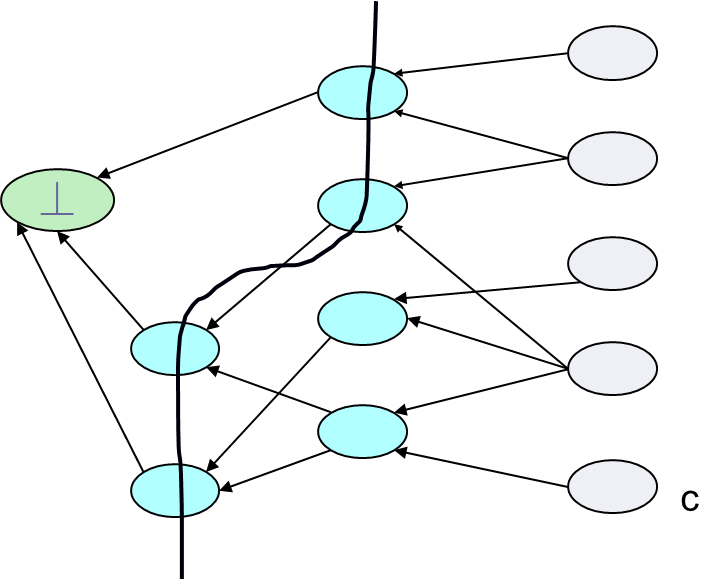
\includegraphics[height=35mm, width = 50mm]{pf.png}
\end{minipage}
&
\begin{minipage}{8 cm}
\includegraphics[height=35mm, width = 50mm]{picture1.png}
\end{minipage}
\\
(a) & (b)\\
\end{tabular}
\caption{(a) The clauses in every vertex cut of an unsatisfiability proof must be unsatisfiable, since together they imply the empty clause
(b) consequently, any assignment that satisfies $\Psi \setminus cone(c,\Pr)$ (the clauses within the dashed polygon) \emph{cannot} satisfy clauses
that appear in all paths of $cone(c,\Pr)$:
otherwise a vertex cut can be satisfied. In this case $c$ and $c1$ are such clauses.
Hence $\Psi \setminus cone(c,\Pr)$ is equisatisfiable to $\Psi \setminus cone(c,\Pr) \cup \lnot c \cup \lnot c1$.
}\label{fig:pf}
\end{center}
\end{figure}

We use this property as follows. Let $P=\left[c_0=c,c_1,\ldots,c_m\right]$ be
a path in the resolution proof starting from a candidate clause $c$.  $P$ is
the \emph{longest unique prefix} if it is the longest path starting at $c$,
such that each $c_i \in P$ has only one child (that is, $c$ participates in
the derivation of one clause only). Clearly clauses in $P$ participate in any
path of $cone(c,\Pr)$, and we can therefore add their negation when checking
$\Psi\setminus cone(c,\Pr)$. This is called \emph{Path strengthening}.
Alg.~\ref{main2} shows a variant of the main algorithm in which path
strengthening has been applied: each invocation of the SAT solver is carried
out under the assumptions $\lnot P=\left\{\lnot c_0,\ldots,\lnot
c_m\right\}$. Before each iteration our algorithm attempts to increase the length of $P$
by removing from the resolution proof clauses that are not backward
reachable from the empty clause. Note that whenever $P$ contains clauses
which do not subsume $c$, path strengthening will provide more assumptions to
the solver than \emph{redundancy
removal}~\cite{DBLP:conf/sat/MaarenW08,DBLP:journals/aicom/BelovLM12}, which
is implemented in \muser. Redundancy removal adds the
literals of $\lnot c$ (where $c$ is the candidate clause) as assumptions when
checking the satisfiability of $S \setminus c$. Observe that this is a
special case of path strengthening. Hence path strengthening is expected to
be more efficient than redundancy removal.


% new Alg 4



\begin{algorithm}
\begin{tabular}{lp{8.5 cm}}
{\bf Input:}  & Unsatisfiability proof $\Pr$ of $\Psi$.\\
{\bf Output:} & A MUC of $\Psi$. \\
\end{tabular} \\
\vspace {0.3 cm}
\begin{algorithmic}[1]
\State $IsSAT := false$;
\State $M := P := \emptyset$;
\While {$(true) $}
\If {($IsSAT$)}
\State \label{step-K5}$K := \{c\}$;
\State \label{step-call5}$M := \alg{ERMR} (\Psi, c, M, K, h)$ \Comment{$h$ is the satisfying assignment}
\Else
\If {\label{step-b:if}proof relies on assumptions}  \Comment{In first iteration the condition is false}
\State $\Pr := \Pr \setminus  cone(c,\Pr)$;
\If {\label{step-b:cond} $condition$}  \Comment{Heuristic. See text}
\State \label{step-b:sat1} $\langle IsSAT,\Pr\rangle := \alg{SAT}(\Pr)$; \Comment{guaranteed unsat}
\EndIf
\EndIf
\EndIf
\If {$core(\Pr) = M$} break; \EndIf
\State Choose $c \in (core(\Pr) \setminus M)$;
\State Let $P$ be the longest unique prefix from $c$;
\State \label{step-b:sat}$\langle IsSAT,\Pr\rangle :=  \alg{SAT}(\Pr \setminus cone(c,\Pr), \{\lnot c_i \mid c_i \in P\})$; \Comment{Second parameter is a set of assumptions}
\EndWhile
\State \Return $M$;

\end{algorithmic}
\caption{An improvement of Alg.~\ref{main1} based on path strengthening. In
line~\ref{step-b:sat} the literals defined by $\{\lnot c_i \mid c_i \in P\}$
are assumptions.} \label{main2}
\end{algorithm}


Cut falsifiability-based techniques are not immediately compliant with clause
set refinement, since clause set refinement requires solving \emph{without
assumptions}.
\muser solves this problem for redundancy removal by applying clause set
refinement only when the assumptions are not used in the proof; otherwise it
skips clause set refinement. Our path strengthening algorithm applies clause
set refinement when either the assumptions are not used in the proof, or the following condition holds (line~\ref{step-b:cond}): for a user-given constant $N$, the $N$ latest iterations
were UNSAT and used assumptions, i.e., line~\ref{step-b:cond} was reached in the last $N$ iterations of the loop. This implies that we did not enjoy the benefits of clause set refinement for $N$ iterations, rather we progressed one clause at a time; it is possibly better to pay the price of an additional SAT call (line~\ref{step-b:sat1}) for the benefit of clause-set refinement.

Since path strengthening is based on finding a joint prefix of the proof from
the removed clause $C$, it is not applicable to HLMUC, since in HLMUC we remove
multiple clauses (``roots") each time, which prevents a joint prefix.


\section{Experimental results}
We tested the effect of the nine optimizations with hundreds of industrial problems, as reported next.


\subsection{HLMUC experiments}
\label{sec:experiments} Our tool \tool{hhlmuc} (for Haifa's high-level MUC)
was built, as mentioned earlier, on top of Minisat 2.2. It contains the
algorithm from Sect.~\ref{sec:prelim} and also the technique of~\cite{SY07}
for reducing the amount of required data in the resolution table by using a
reference-counter. 
On top of this we implemented the optimizations that were
described in the previous section, and ran all possible combinations
(excluding the restrictions mentioned in optimization E, and excluding optimization H --- see below a separate experiment with that optimization), on the set used in~\cite{N10} (family `lat-fmcad10' in the tables below), and additional nine families of harder abstraction-refinement benchmarks from Intel.
We removed from the benchmark set instances that could not be solved by any of
the configurations in the given time-out of one hour. This left us with 144
benchmarks, all of which are from the two application domains that were
described in the introduction. This set constitute Intel's contribution to
the benchmarks repository that was used in the SAT competition
dedicated to this problem. The average number of clauses per instance is
2,572,270; the average number of constraints per instance is 3804; and,
finally, the average number of clauses in the high-level constraints per instance is 96568
(25.3 clauses per constraint), which is approximately 6\% of the clauses. All
experiments were ran on Intel\textregistered\ Xeon\textregistered\ machines
with 4Ghz CPU frequency and 32Gb of memory.


Table~\ref{ta:1} shows run time results for selected
configurations.\footnote{The tool and the full set of results, including a
comparison to MUC tools (which does not appear here) can be downloaded
from~\cite{RS11-URL}.} The second column (``Base") refers to our starting
point, namely an implementation of Alg.~\ref{alg:A2}. One may observe that the best result is achieved when combining the first six optimizations, whereas the seventh slightly increases the overall run-time.



We also compared our results to assumptions-based minimization. We tried two methods. In the simple
method, a constraint is added to the MUC (line~\ref{step:M2} in
Alg.~\ref{alg:A2}) by setting its associated selector variable to true; in
the improved method the same effect is achieved by adding a unit clause
asserting this literal to \true. Similarly, in the simple method an
environment assumption is removed from the formula (line~\ref{step:remove2}
in Alg.~\ref{alg:A2}) by setting its associated selector to \false; In the
improved method the same effect is achieved by adding a unit clause asserting
this literal to \false. The improved method is better empirically apparently
because the unit clause invokes a simplification step in decision level 0,
which removes the selector variable and erases some clauses. The results we
witnessed with the two methods appear in the last two columns of the table.
Overall the combination of optimizations achieve a reduction of 55\% in run
time comparing to our starting point, and a reduction of 28\% comparing to
the assumptions-based method.


All the presented methods can be affected by the order in which constraints
are removed in line~\ref{step:Hk2} of Alg.~\ref{alg:A2}. We therefore tried three different
arbitrary removal orders in each case. Empirically this hardly had an effect
on the average run-time when using the resolution-based methods, whereas it
had some effect when using the assumption-based methods. The table below
represents the best overall run times among the different orders we tried
(i.e., we present the results that together have the minimum run-time).
Regarding the size of the resulting core, the different arbitrary orders had
inconsistent effect, as expected, but the order referred to in optimization
G had a non-negligible positive effect on the size of the core, as will
be shown momentarily.


\begin{table}
\begin{center}
\scalebox{0.95}{
\begin{tabular}{|l|c|c|c|c|c|c|c|c|c|c|}\hline
Bench.	& \multicolumn{8}{c|}{Resolution-based}	&        \multicolumn{2}{c|}{Assum.-based} \\ \cline{2-11}
family	&  Base  	&  A	    &  AB    	&  ABC   	&  ABCE  	& A--E 	    &  A--F	    & A--G	&  	    	 &  units \\ \hline
latch1      &  2001		&  1604		&  660		&  465		&  570		&  575		&  425		& 423	&  819		 &   798 \\
gate1	    &  3747		&  1403		&  705		&  636		&  620		&  579		&  490		& 477	&  856		 &   855 \\
latch2      &  9113		&  5915		&  6636		&  6116		&  5685		&  5656		&  2424		& 2370	&  8153		&   8043 \\
latch3      &  348		&  293		&  274		&  274		&  283		&  275		&  262		& 200	&  236		 &   236 \\
latch4     	&  769		&  529		&  506		&  457		&  467		&  455		&  443		& 379	&  504		&   521 \\
latch5     	&  1103		&  820		&  735		&  657		&  678		&  630		&  632		& 625	&  747		&   689 \\
fm-d10	&  785		&  457		&  445		&  451		&  435		&  435		&  400		& 394	&  417		&   425 \\
latch6      &  8868		&  5456		&  5329		&  5188		&  5007		&  5006		&  4948		& 4943	&  5322		&   5279 \\
latch7	    &  9956		&  7050		&  5719		&  5244		&  5094		&  5096		&  5302		& 5286	&  5688		&   5652 \\
latch8     &  8223		&  7946		&  5673		&  6133		&  5459		&  5420		&  5127		& 5587	&  8004		&   5534 \\ \hline
Total	&  44913	&  31473	&  26682	&  25621	&  24298	&  24127	& {\bf 20453}& 20684 &  30746	&   28032\\ \hline
\end{tabular}
}
\vspace{0.1 cm}
\caption{Summary of run-time results by family (144 instances all together). `fm-d10' is the `lat-fmcad10' family. }\label{ta:1}
\end{center}
\end{table}


Next, in Table~\ref{ta:2}, we consider the size of the resulting HLMUC. The configuration that
achieves the best run-time (A--F) achieves the second smallest HLMUC, whereas
the second best configuration in terms of run time (A--G) achieves the
smallest core. If a solver timed-out in our experiments, we considered its
latest computed core, i.e., the set $M \cup HLC$. If a solver did
not finish even the first iteration, then we considered the entire set of
clauses in $HLC$ as its achieved core. This policy, which reflects the way
such cores are used, explains the different results of strategies that are
supposed to be equivalent with respect to the size of the core. For example,
the partial-resolution proof optimization (A) does not remove more
clauses than `Base', but since the latter is generally slower, it times-out
more times and hence its core count is larger. The `TO' row contains the
number of such time-outs with each configuration.

%\samepage{
\begin{table}
\begin{center}
\begin{tabular}{|l|c|c|c|c|c|c|c|c|c|c|}\hline
Bench.	& \multicolumn{8}{c|}{Resolution-based}	&        \multicolumn{2}{c|}{Assum.-based} \\ \cline{2-11}
family	&  Base		&    A		&  AB    		&  ABC   		&  ABCE  		& A--E	& A-F	& A-G	 &  &  units	 \\ \hline
latch1      &  41		&  41		&  41		&  41		&  42		&  42		&  41		& 42	&  52		&   45	\\
gate1	    &  1143		&  1210		&  1089		&  568		&  1029		&  1029		&  870		& 901	&  618		&   1192	\\
latch2    	&  5887		&  2851		&  127		&  3040		&  2851		&  2851		&  131		& 129	&  3782		&   4165	\\
latch3      &  168		&  202		&  202		&  199		&  211		&  211		&  208		& 123	&  140		&   132	\\
latch4 		&  236		&  237		&  248		&  236		&  238		&  238		&  237		& 162	&  177		&   217	 \\
latch5 		&  224		&  266		&  266		&  206		&  206		&  206		&  220		& 222	&  222		&   223	 \\
fm-d10	&  577		&  456		&  456		&  489		&  540		&  540		&  453		& 454	&  457		&   450	 \\
latch6      &  2550		&  2502		&  2502		&  2490		&  2490		&  2490		&  2480		& 2480	&  2463		&   2502	\\
latch7	    &  2578		&  322		&  585		&  253		&  154		&  154		&  211		& 204	&  304		&   287	\\
latch8      &  5591		&  615		&  2867		&  393		&  344		&  344		&  371		& 373	&  2887		&   2877	\\ \hline
TO          & 8         & 5	        & 3	        & 3         & 2         & 2         & 2         & 2     & 6         & 5 \\ \hline
Total	    &  18995	&  8702		&  8383		&  7915		&  8105		&  8105		&  5222		& {\bf 5090}& 11102 &   12090	\\ \hline

\end{tabular}
\vspace{0.1 cm} \caption{Summary of the size of the HLMUC by family. The `TO'
row indicates the number of time-outs.}\label{ta:2}
\end{center}
\end{table}


\paragraph{The effect of rotation (H), and a comparison to \muser}
We recently conducted another set of experiments, this time with the 197 GMUS competition benchmarks in order to compare ourselves to the latest version of \muser and also for checking the effect of optimization H (eager rotation) which we recently implemented. The experiments were conducted on Intel$\circledR$ Xeon$\circledR$ CPU E5-2670 processors with 2.60GHz CPU frequency and having 64Gb of memory.
The results are:
\begin{itemize}
\item \haifahlmuc with optimization  A -- G: 28187 sec.
\item \haifahlmuc with optimization  A -- H: 11483 sec.
\item \muser (default configuration, which includes rotation): 20440 sec.
\end{itemize}
Hence the winning strategy, which is now the default of \haifahlmuc, is  A -- H.
%
A detailed comparison of \haifahlmuc to \muser can be seen in Fig.~\ref{fig:hvsmuser}.
\begin{figure}
\begin{center}
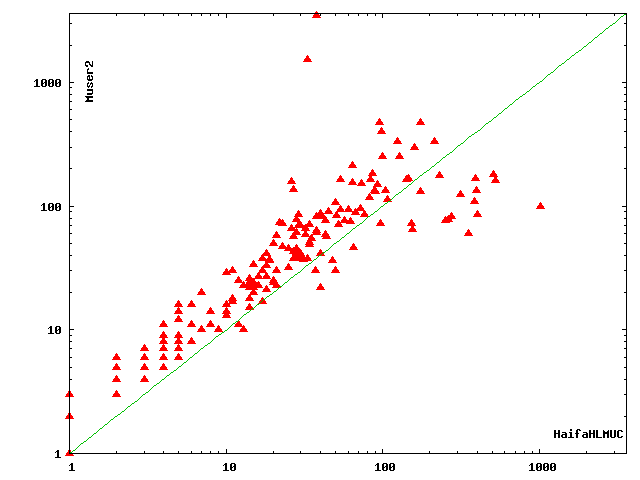
\includegraphics[height=71mm, width = 75mm]{hsatVsMuser2.png}
\caption{Comparing \haifahlmuc to \muser (Nov. 2014) with the 2011 GMUS competition benchmarks.}\label{fig:hvsmuser}
\end{center}
\end{figure}



\subsection{MUC experiments}
\label{sec:er}

%[* add data on core reduction, and be more specific about the impact of optimizations E,F *]
We checked the impact of our algorithms when applied to
the 295 instances used for the MUC track of the SAT 2011 competition. For the
experiments we used machines with 32Gb of memory running Intel$\circledR$
Xeon$\circledR$     processors with 3Ghz CPU frequency. The time-out was set to
1800 sec. The implementation was done in \haifamuc. We refer to a
configuration of \haifamuc that implements the deletion-based algorithm with
incremental SAT and clause set refinement as Base.  We compare our tool to
the latest version of \muser~\cite{BelovM12} and \muserabr~\cite{LB13}.
\muser applies the basic deletion-based approach to MUC extraction, described in Section~\ref{sec:prelim}, using assumptions to keep track of dependencies. It enhances the basic deletion-based approach by rotation and redundancy removal, which we described as part of optimizations H and I. \muserabr is an extension of \muser: it replaces blocks of assumptions with new variables and stores the dependencies between them. This technique is similar in essence to our optimization  A  (instead of storing resolution information, it stores these dependencies). In addition, \muserabr applies clause minimization selectively, which is similar to our optimization  B. Extended experimental data is available from the second author's home page.
%\footnote{The version of \haifamuc that won the SAT 2011 competition is Base enhanced by optimizations A + D, described in Sec.~\ref{sec:opt}.}


\begin{table}
%\begin{center}
%\scriptsize
\footnotesize
\begin{tabular}{|l|lllllllll|}
\hline
&Base&rot&erot&erot\_ &erot\_&erot\_&erot\_ &\textbf{erot\_}    &\textbf{erot\_}\\
&    &   &    &  AD   & ABD  & AB2D & AB2CD & \textbf{AB2CD\_rr}& \textbf{AB2CD\_ps20}  \\
\hline
Time&93931&48018&44335&36295&37798&32968&32918&30800&\textbf{27263}\\
Unsolved&30&12&10&8&13&8&8&6&\textbf{4}\\
\hline
\end{tabular}

\vspace{0.1 cm}

\begin{tabular}{|l|ll|} \hline
        & \muser&\muserabr \\ \hline
Time    &59502  &40485 \\
Unsolved&17     &8 \\
\hline
\end{tabular}

%\small
\caption{\strut Total run-time in sec. and number of unsolved instances for various solvers, when applied to the 295 instances from the 2011 MUC competition, excluding 12 instances which were not solved by any of the solvers (the time-out value of 1800 sec. was added to the run-time when a memory-out occurred). Base is defined in Sect.~\ref{sec:er}, rot = Base+rotation, erot = Base+eager rotation.  A,  B,  C, and D correspond to the optimizations defined in Sect.~\ref{sec:opt}. `2' in AB2CD means that the optimization was invoked after the 2nd satisfiable result.  `rr' refers to redundancy removal combined with clause set refinement using \muser's scheme, described in Sect.~\ref{sec:opt}. `ps20' means that path strengthening with $N=20$ was applied as described in Sect.~\ref{sec:opt}.}\label{tab:results}
%\end{center}
\end{table}


Table.~\ref{tab:results} summarizes the main results. Several observations are in order: 1) rotation is very useful; 2) eager rotation is effective; 3) optimizations A and D are useful, while optimization B is beneficial only if delayed until the second satisfiable iteration (2 being the optimal value, based on experiments); 4) path strengthening (with $N$=20, 20 being the optimal value experimentally) is more beneficial than redundancy removal, and finally 5) \haifamuc, enhanced by all our algorithms, is \xvsmuser faster than \muser  and solves \tvsmuser more instances, and is \xvsabr faster than \muserabr and solves \tvsabr more instances. \haifamuc is faster than \muserabr on 196 instances, while \muserabr is faster than \haifamuc on 15 instances. Fig.~\ref{fig:hm} compares \haifamuc to \muserabr and Fig.~\ref{fig:cactus} shows a cactus plot comparing Base, \muser, \muserabr and the new best configuration of \haifamuc.

\begin{figure}
%\vspace{-0.5 cm}
\begin{center}
%\begin{tabular}{ll}
%\begin{minipage}{9.0 cm}
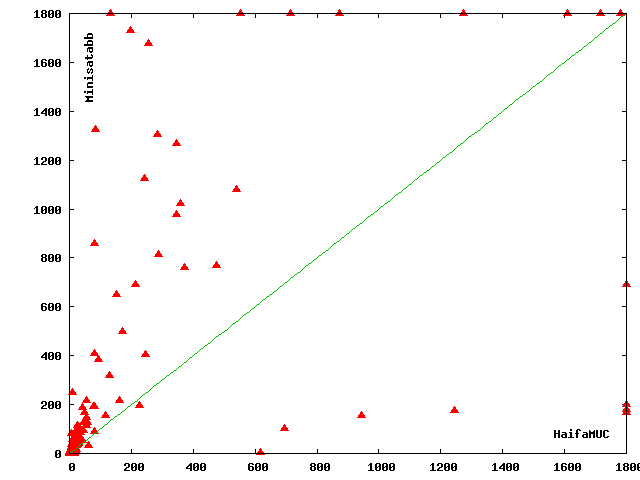
\includegraphics[height=71mm, width = 75mm]{HaifaMUC_vs_Minisatabb.png}
%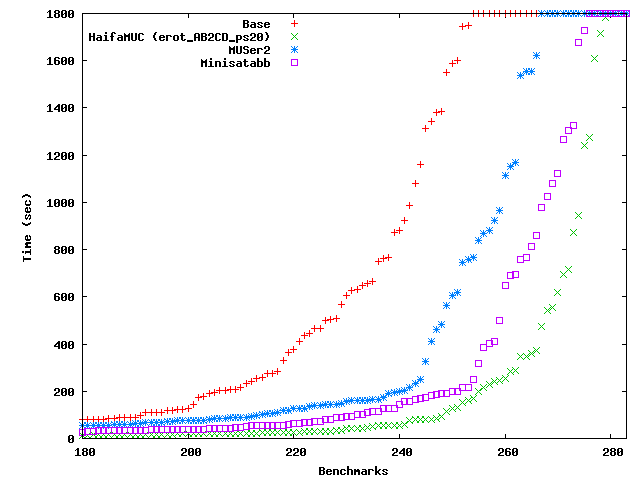
\includegraphics[scale=0.75]{graph.png}
\caption{Direct comparison of the new best configuration of \haifamuc erot\_AB2CD\_ps20 (X-Axis) and \muserabr (Y-Axis). \vspace{0.5 cm}}
\label{fig:hm}
\end{center}
%\end{minipage}
%&
\end{figure}
\begin{figure}
%\begin{minipage}{8.5 cm}
\begin{center}
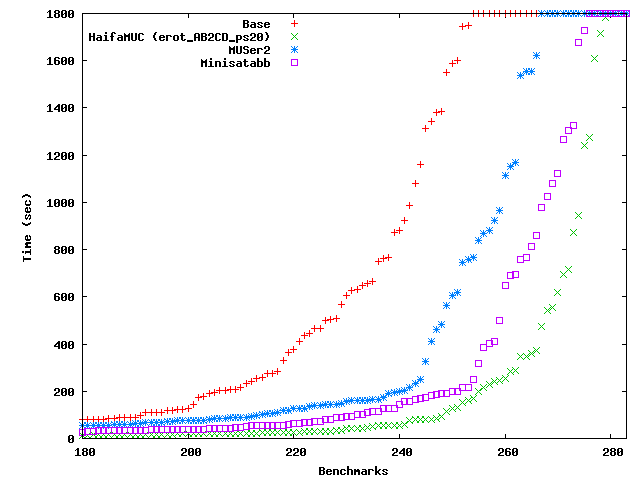
\includegraphics[height=59mm, width = 100mm]{graph.png}
%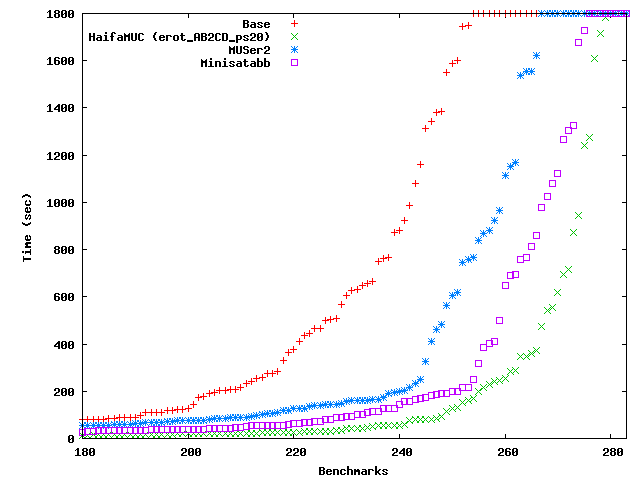
\includegraphics[scale=0.75]{graph.png}
\caption{Comparison of Base, \muser, \muserabr, and the new best configuration of \haifamuc erot\_AB2CD\_ps20. The graph shows the number of solved instances (X-Axis) per time-out in seconds (Y-Axis)  for each solver.}
\label{fig:cactus}
%\end{minipage}
\end{center}
%\end{tabular}
\end{figure}





\section{Summary and future work}
We presented a basic deletion-based method for finding high-level unsat cores. Earlier methods were based on retrieving first a minimal core, and then deriving from it a high-level core, which means that it was not necessarily minimal.
We also presented nine optimizations to MUC- and HLMUC-extraction, although not all
apply to both goals. Some of these optimizations bias the search itself towards a minimal core. These are the main techniques underlying our tools
\haifamuc and \haifahlmuc, which are currently the fastest of their kind.

A straight-forward direction for future research is to migrate some of the
suggested optimizations to the assumptions-based approach. Related SAT
problems may also benefit from these methods. First, it is possible that
general SAT solving can be improved with some combination of optimizations
E and F. Second, the same techniques can potentially expedite
other methods in which the SAT component needs to extract only partial
information from the resolution proof, like interpolation-based model
checking~\cite{M03}. In interpolation only a small part of the proof
% (the `A' side, as defined in the above reference, and those clauses derived from the `B' side that are resolved with their descendants),
is necessary in order to generate the interpolant, so it should be useful to explore
possibilities to minimize that part and decrease the overall run time with
variants of the methods suggested here.


\bibliographystyle{plainbv}
\bibliography{biblio}
\end{document}
